\documentclass[12pt,letterpaper]{article}
\usepackage[utf8]{inputenc}
\usepackage[english]{babel}
\usepackage{ifpdf}
\makeatletter
\@namedef{ver@thumbpdf.sty}{}
\makeatother
\usepackage{mla}
\usepackage{todonotes}

\usepackage[pass]{geometry}
\usepackage[hidelinks]{hyperref}
\urlstyle{same}

\usepackage{csquotes}
\usepackage[style=mla-new,backend=biber]{biblatex}
\addbibresource{essay-4.bib}
\DeclareBibliographyAlias{misc}{article}

\usepackage{textcomp}
\usepackage{gensymb}
\newcommand*{\aprime}{^{\prime}\mkern-1.2mu}
\newcommand*{\dprime}{^{\prime\prime}\mkern-1.2mu}

\usepackage{amsmath}
\usepackage{graphicx}
\usepackage{float}
\usepackage{subcaption}

\newenvironment{absnobreak}
{\par\nobreak\vfil\penalty0\vfilneg%
\vtop\bgroup}
{\par\xdef\tpd{\the\prevdepth}\egroup%
\prevdepth=\tpd}

\begin{document}
\begin{mla}{Bernardo}{Meurer}{Professor Eckford-Prossor}{English 111 H}{April 16, 2018}{The Age of Nothing}
    I took a train this weekend, from Santa Barbara down to Los Angeles and, despite Amtrak's usual punctuality, I found myself enjoying the trip. The railroad is quite scenic, until it goes into Oxnard, and a number of farms start appearing out of nowhere, with irrigation so plentiful one would never judge California to be in a drought. In one of these fields there were a few dozen workers picking something that I made out to be tomatoes, but considering my sight could be anything, one by one. Here it struck me, some of those workers could have been working there for over a decade, in some sense farming, and yet I wondered whether they had ever touched the soil they step on and live off with their bare hands. Even more so, I wondered whether whomever owns the farm ever touched on the soil they reap from; has anyone who works there? I wonder when was the last time one of them grabbed the soil to feel its moisture, if any of them ever tasted the soil for alkalinity; I doubt it.

    In that farm, of course, the workers only reap what they have not sown; a machine planted the seeds after all. Seeds which, most likely, came from a lab, carefully engineered to germinate into sterile plants. Fake seeds, planted by a machine, operated by someone who knows only the gauges and knobs of it, picked by men who know only how to pick, eaten by people who get it, cleaned, sterilized, pulverized, from a box; where did the farmer go? He's gone, of course; not fast enough, not productive enough, not scalable. Somehow along the way we seem to have lost a fundamental connection with the self; we seem to have forgotten that what we do should be meaningful, if not to others than to ourselves.

    \begin{figure}[H]
        \centering
        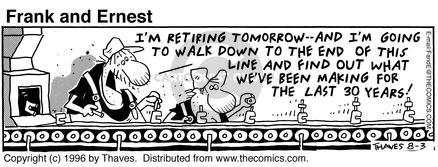
\includegraphics{assembly.jpg}
    \end{figure}

    In one form or another, the symptoms of this amnesia of meaning have been around since the 19th century, becoming truly noticeable in the start of the Victorian Era. Somehow this aesthetic smokescreen began raising, clouding our vision and perception. Things had to be clean, perfect and homogeneous, relationships had to be friction-less, stable, and beautiful. There was no concern for the inherent impossibility of these desires, a machine, a pill, a specialist; \emph{Fiant pilulae et pereat mundus} \autocite[1]{schopenhauer_2009}. What does one do, then, when something doesn't meet said requirements, if not force them into the frame we desire. Eliot writes, in ``II.~A Game of Chess'':
    \begin{blocks}
        ``What is that noise?''\\
        \hspace{72pt}The wind under the door.\\
        ``What is that noise now? What is the wind doing?''\\
        \hspace{72pt}Nothing again nothing.\hfill 120\\
        \hspace{180pt}``Do\\
        ``You know nothing? Do you see nothing? Do you remember\\
        ``Nothing?''\\
        \hspace{20pt}I remember\\
        Those are pearls that were his eyes.\hfill 125\\
        ``Are you alive, or not? Is there nothing in your head?''\\
        \hspace{212pt}But\\
        O O O O that Shakespeherian Rag---\\
        It’s so elegant\\
        So intelligent\hfill 130\\~\\
        ``What shall I do now? What shall I do?\\
        ``I shall rush out as I am, and walk the street\\
        ``With my hair down, so. What shall we do tomorrow?\\
        ``What shall we ever do?''\\
        \hspace{67pt}The hot water at ten.\hfill 135\\
        And if it rains, a closed car at four.\\
        And we shall play a game of chess,\\
        Pressing lidless eyes and waiting for a knock upon the door.\\
        \autocite[9]{eliot_2001}~\phantom{''~''~''~''~''}% Hack for the unequal quotes
    \end{blocks}
    The woman in this ``scene'' is clearly altered, drugged, and yet there is this overarching sense of utter normality in the situation. The (supposed) husband isn't worried, or surprised, this is a day like any other, this is just how things are. Yet it is clear that this perfect, clean, faultless relationship does not truly exist, it's only an illusion, it's nothing.

    Unfortunately, we haven't only lost ourselves in work and love, but this meaninglessness permeates modern life like a plague. People's social lives revolve around digital points, likes, loves, given to them by digital friends. We take pictures not to reminisce and long but to show our lives to mutually uninterested parties. We say vacuous words to endless pits of digital text wanting only to be heard. The message is secondary, what matters is that you have \textit{a} message, and everyone
    must know it, and see it, and like it, and share it. People talk endlessly on TV sets, YouTube, Facebook, and endless other channels; but what do they say?

    It is said that Flaubert wanted to write a romance about nothing, had he lived in our time he would've had great success. We live in a conjuncture so bizarre even our money is meaningless; what is a dollar after all? It's nothing, it's worth what people decide it to be. A dollar doesn't represent any physical quantity proper, not even the value of the paper that makes it; most of it is purely digital. Maybe I'm too simple-minded, but I find this existence to be overwhelming, somehow we have
    enslaved ourselves but we can't see it. I don't think Eliot could have predicted how deeply buried into nothing we would be, but he clearly saw the beginning of this loss of meaning coming.

    The austerity we live in is an intellectual and emotional one. Our quality of live improves by the day, and yet we feel lonely, and hatred towards what's different; it seems somehow the more we know and the more advanced we are, the more ignorant we become.
    F.R. Leavis, in ``The Significance of the Modern Waste Land,'' writes: ``The remoteness of the civilization celebrated in \emph{The Waste Land} from the natural rhythms is brought out \ldots by the anthropological theme \ldots Sex here is sterile, breeding not life and fulfilment but disgust, accidia and unanswerable questions'' \autocite[Eliot 174]{eliot_2001}.
    This remoteness, this sterility, is precisely what I am describing, perhaps it is fair to say we've genetically engineered the seeds to be like us, and our reality.

    In ``I.~The Burial of the Dead,'' of \textit{The Waste Land} Eliot writes:
    \begin{blocks}
        Unreal City,\hfill 60\\
        Under the brown fog of a winter dawn,\\
        A crowd flowed over London Bridge, so many,\\
        I had not thought death had undone so many.\\
        Sighs, short and infrequent, were exhaled,\\
        And each man fixed his eyes before his feet.\hfill 65\\
        Flowed up the hill and down King William Street,\\
        To where Saint Mary Woolnoth kept the hours\\
        With a dead sound on the final stroke of nine.\\
        \(\lbrack\ldots\rbrack \)\hfill \autocite[7]{eliot_2001}
    \end{blocks}
    In this stanza the ``crowd'' of undead refers to the huge numbers of proletariat-class workers marching towards their respective factories. Eliot's characterization of them as an undead crowd is extremely accurate, and is unchanged today. The same line could apply today, if only we replace ``feet'' for ``screen''; feet are too gruesome after all. Again, somehow we've allowed death to undo us all, and endless crowd of undead men and women, of which I am a part of; how did we get here? Where has our sense of wonder and dazzle gone?

    Although it may seem like the question of meaninglessness is only secondary in the poem, quite the opposite is true. This motif is protagonist in the poem, not so much by taking over the content, but rather by \emph{how} the content is presented, in a quasi-wittgensteinian sense. Since the means are themselves the message, meaningless takes a silent control of the poem.
    In ``An Anatomy of Melancholy,'' Conrad Aiken argues that ``the poem succeeds \ldots by virtue of its incoherence, not of its plan; by virtue of it's ambiguities, not its explanations. Its incoherence is a virtue because its `donnée' is incoherence'' \autocite[Eliot 152]{eliot_2001}. I think the incoherence of the poem is a subliminal message, which speaks about the message of our era itself.

    For the last two hundred years or so we have lived in a post-enchantment world \autocite[12]{jenkins_2012}. Western society has been mostly disenchanted; in a world where everything is known by someone there is no need, or space, for magic or lore of any kind. It is because of this that religion, for example, has been on a slow but steady decline, allowing us to hear such pearls as ``I am morally Christian,'' which in non-euphemism means ``I don't believe in fairy tales, but I like the Christian moral-framework.'' How could they be Christian, of course there is no God, there is only us; alone in our arrogance.

    Now, if there is no space for non-logic, and there is this overarching certainty that whatever it is that we may wonder about is already known by \emph{someone}, why wonder at all? Why should people waste their energy and time watching water go down the drain in a vortex and thinking ``Hmm, odd''? Worst even, for those that do consider it, why employ time into trying to conjecture a reason, when Google knows it immediately? The answer to these questions may not be obvious, but it
    should; because it's what makes us Human. What is the defining Human characteristic if not our ability, and our impulse, to reason. How else could we have gotten so far, so developed, so quickly if not by relentlessly questioning.

    It's no wonder Eliot calls us a crowd undone by death, we have lost that which makes us living humans. We've allowed others to convince us that things are too complex to be understood, we've allowed ourselves to delegate thinking to others, and reject our personhood; we must reclaim it. Let us allow the one who sows to reap as well, for the worker to ponder and reflect on his work. Let us allow ourselves to be fascinated by everyday life, and to wonder, and err, about the reasons of things. Let us forget about the numerology in our memories, the shackles of the countably invisible approval of others, and simply enjoy the moments we live in. We must allow ourselves to come back to life, and be human again.
    \newpage
    \printbibliography{}
\end{mla}
\end{document}
